\documentclass[11pt]{article}
\usepackage[utf8]{inputenc}
\usepackage{longtable}
\usepackage{color}
\usepackage{multirow}
\usepackage{hyperref}
\usepackage{setspace}
%\doublespacing

\renewcommand*{\sectionautorefname}{Section} 

\title{Policy emergence model 4.0 - Formalisation \\ With Schelling model}
\author{Raphael Klein}

\usepackage{natbib}
\usepackage{graphicx}
\usepackage[labelfont=bf]{caption} 	% Make captions bold (Figure & Table)
\usepackage{subfig}	
\usepackage{amsmath}
\usepackage{hyperref}
%\usepackage[section]{placeins}

\providecommand{\keywords}[1]{\textbf{Keywords:} #1}

\begin{document}

\maketitle

%\begin{center}
%Word count: 9300 words
%\end{center}


\tableofcontents

[The paper for the formalisation should be transformed into an ODD paper]

The ODD template states the following:
1. Purpose: what is the purpose of the model?
2. Entities, state variables and scales: What kinds of entities are in the model? By what state variables, or attributes, are these entities characterized? What are the temporal and spatial resolutions and extents of the model?
	- Agents/individuals [one type of agent here]
	- Spatial units (grid cells) [there is a grid where the agents are situated]
	- Environment [ultimately, the environment will be the policy making model]
	- Collectives [not present in the Schelling model]
3. Process overview and scheduling: Who (i.e., what entity) does what, and in what order? When are state variables updated? How is time modelled, as discrete steps or as a continuum over which both continuous processes and discrete events can occur? Except for very simple schedules, one should use pseudo-code to describe the schedule in every detail, so that the model can be reimplemented from this code. Ideally, the pseudo-code corresponds fully to the actual code used in the program implementing the ABM.
4. Design concepts
5. Initialisation: What is the initial state of the model world, i.e., at time t = 0 of a simulation run? In detail, how many entities of what type are there initially, and what are the exact values of their state variables (or how were they set stochastically)? Is initialization always the same, or is it allowed to vary among simulations? Are the initial values chosen arbitrarily or based on data? References to those data should be provided.
6. Input data: Does the model use input from external sources such as data files or other models to represent processes that change over time?
7. Submodels: What, in detail, are the submodels that represent the processes listed in ?Process overview and scheduling?? What are the model parameters, their dimensions, and reference values? How were submodels designed or chosen, and how were they parameterized and then tested? [There are none here]



%%%%%%%%%%%%%%%%%%%%%%%%%%%%%%%%%%%%%%%%%%%%%%%%%%%%%%%%%%%%%%%%%%
\section{The agents}
\label{sec:agents}
%%%%%%%%%%%%%%%%%%%%%%%%%%%%%%%%%%%

Five types of permanent agents and one temporary agent are considered in the policy process. These are divided in two main categories: the active agents which have to strategise and the passive agents  that perform mandatory actions.

%%%%%%%%%%%%%%%%%%%%%%%%%%%%%%%%%%%
%- THE AGENTS - Active agents
\subsection{Active agents}
\label{ssec:activeAgents}

The active agents are the policy makers, the policy entrepreneurs and the external parties. Note that the external parties also have a passive role in which relay information on the environment to the truth agent, to the policy makers, the policy entrepreneurs, other external parties, and the electorate. This is considered to be a passive action as it does not require decision making.

The active agent's attributes are given as follows:

\begin{enumerate}

\item The \emph{active agent} is represented as an 10-tuple given by \texttt{agent = (ID, type, issueTree, policyTree, affiliation, resources, category)} where
\texttt{ID} is the unique ID of the agent,
\texttt{type} is the choice of agent type, 
\texttt{issueTree} is the agent's personalised issue tree, 
\texttt{policyTree} is the agent's personalised policy tree, 
\texttt{affiliation} is the political entity the agent identifies with,  
\texttt{resources} is the agent's resources (a relative value), and 
\texttt{category} outline the agent's focus on either issues or policies.

\item A \emph{type} corresponds to a choice of agent. This can either be a policy maker, a policy entrepreneur or an external party. Depending on the type of agent, the actions will change from one agent to another.

\item The \emph{issue tree} is made of two main parts: the agent's own issue tree, and the issue tree of all other agents based on the agent's perceived knowledge of their issues (later referred as partial knowledge). The entire \emph{issue tree} structure is therefore a list of issue trees which is as long as the number of agents present in the model. The details of the tree itself are provided in \autoref{sec:beliefSystem}.

\item The \emph{policy tree} is similar to the issue tree but for policies. This is detailed in \autoref{sec:beliefSystem}.

\item The \emph{resources} are represented as a decimal on the interval [0, 1]. Resources are distributed to the agents based on their affiliation and on that affiliation's representation within the model. These resources are used by the agent to perform actions on other agents. The resources are relative amongst all agents.

\item The \emph{category} helps define whether an agent will be issue or policy focused. This can be an input if an agent is well known for having a certain predisposition. If this is not the case, the category is defined based on the preferences of the agent in his/her issue and policy trees.

\end{enumerate}

%%%%%%%%%%%%%%%%%%%%%%%%%%%%%%%%%%%
%- THE AGENTS - Passive agents
\subsection{Passive agents}
\label{ssec:passiveAgents}

The main passive agent is the truth agent and the electorate. It performs passive actions (without any decision making power).

\emph{The truth agent: } The truth agent is an agent not mentioned in the conceptualisation but required for the formalisation. This agent helps make the link between the world and the agents within the model. It gathers all the states of the world and provides them, as they are, to the external parties. The only attribute of the truth agent is the issue tree. This is a different one that for the active agents. It only contains the overall similar structure without any causal relations. Furthermore, it only contains the beliefs for each of the issues.


%%%%%%%%%%%%%%%%%%%%%%%%%%%%%%%%%%%%%%%%%%%%%%%%%%%%%%%%%%%%%%%%%%
\section{The belief system}
\label{sec:beliefSystem}
%%%%%%%%%%%%%%%%%%%%%%%%%%%%%%%%%%%

The belief system of the agents is split in two parts: the issue tree and the policy tree. The issue tree provides information on the beliefs of the agents on all of the issues present in the socio-technical model while the policy tree provides information on the agents' beliefs on the policies.

%%%%%%%%%%%%%%%%%%%%%%%%%%%%%%%%%%%
%- THE BELIEF SYSTEM - The issue tree
\subsection{The issue tree}
\label{ssec:issueTree}

The issue tree is made of two main components: issues and causal relations. The issues are categorised in three hierarchical layers: the deep core issues (the top layer), the policy core issues (the middle layer) and the secondary issues (the bottom layer)\citep{sabatier1998advocacy}. Secondary issues are linked to policy core issues through causal relations while policy core issues are linked to deep core beliefs through different causal relations. The representation of the issue tree is shown in \autoref{fig:IssueTree-01}.

\begin{figure}
\centering
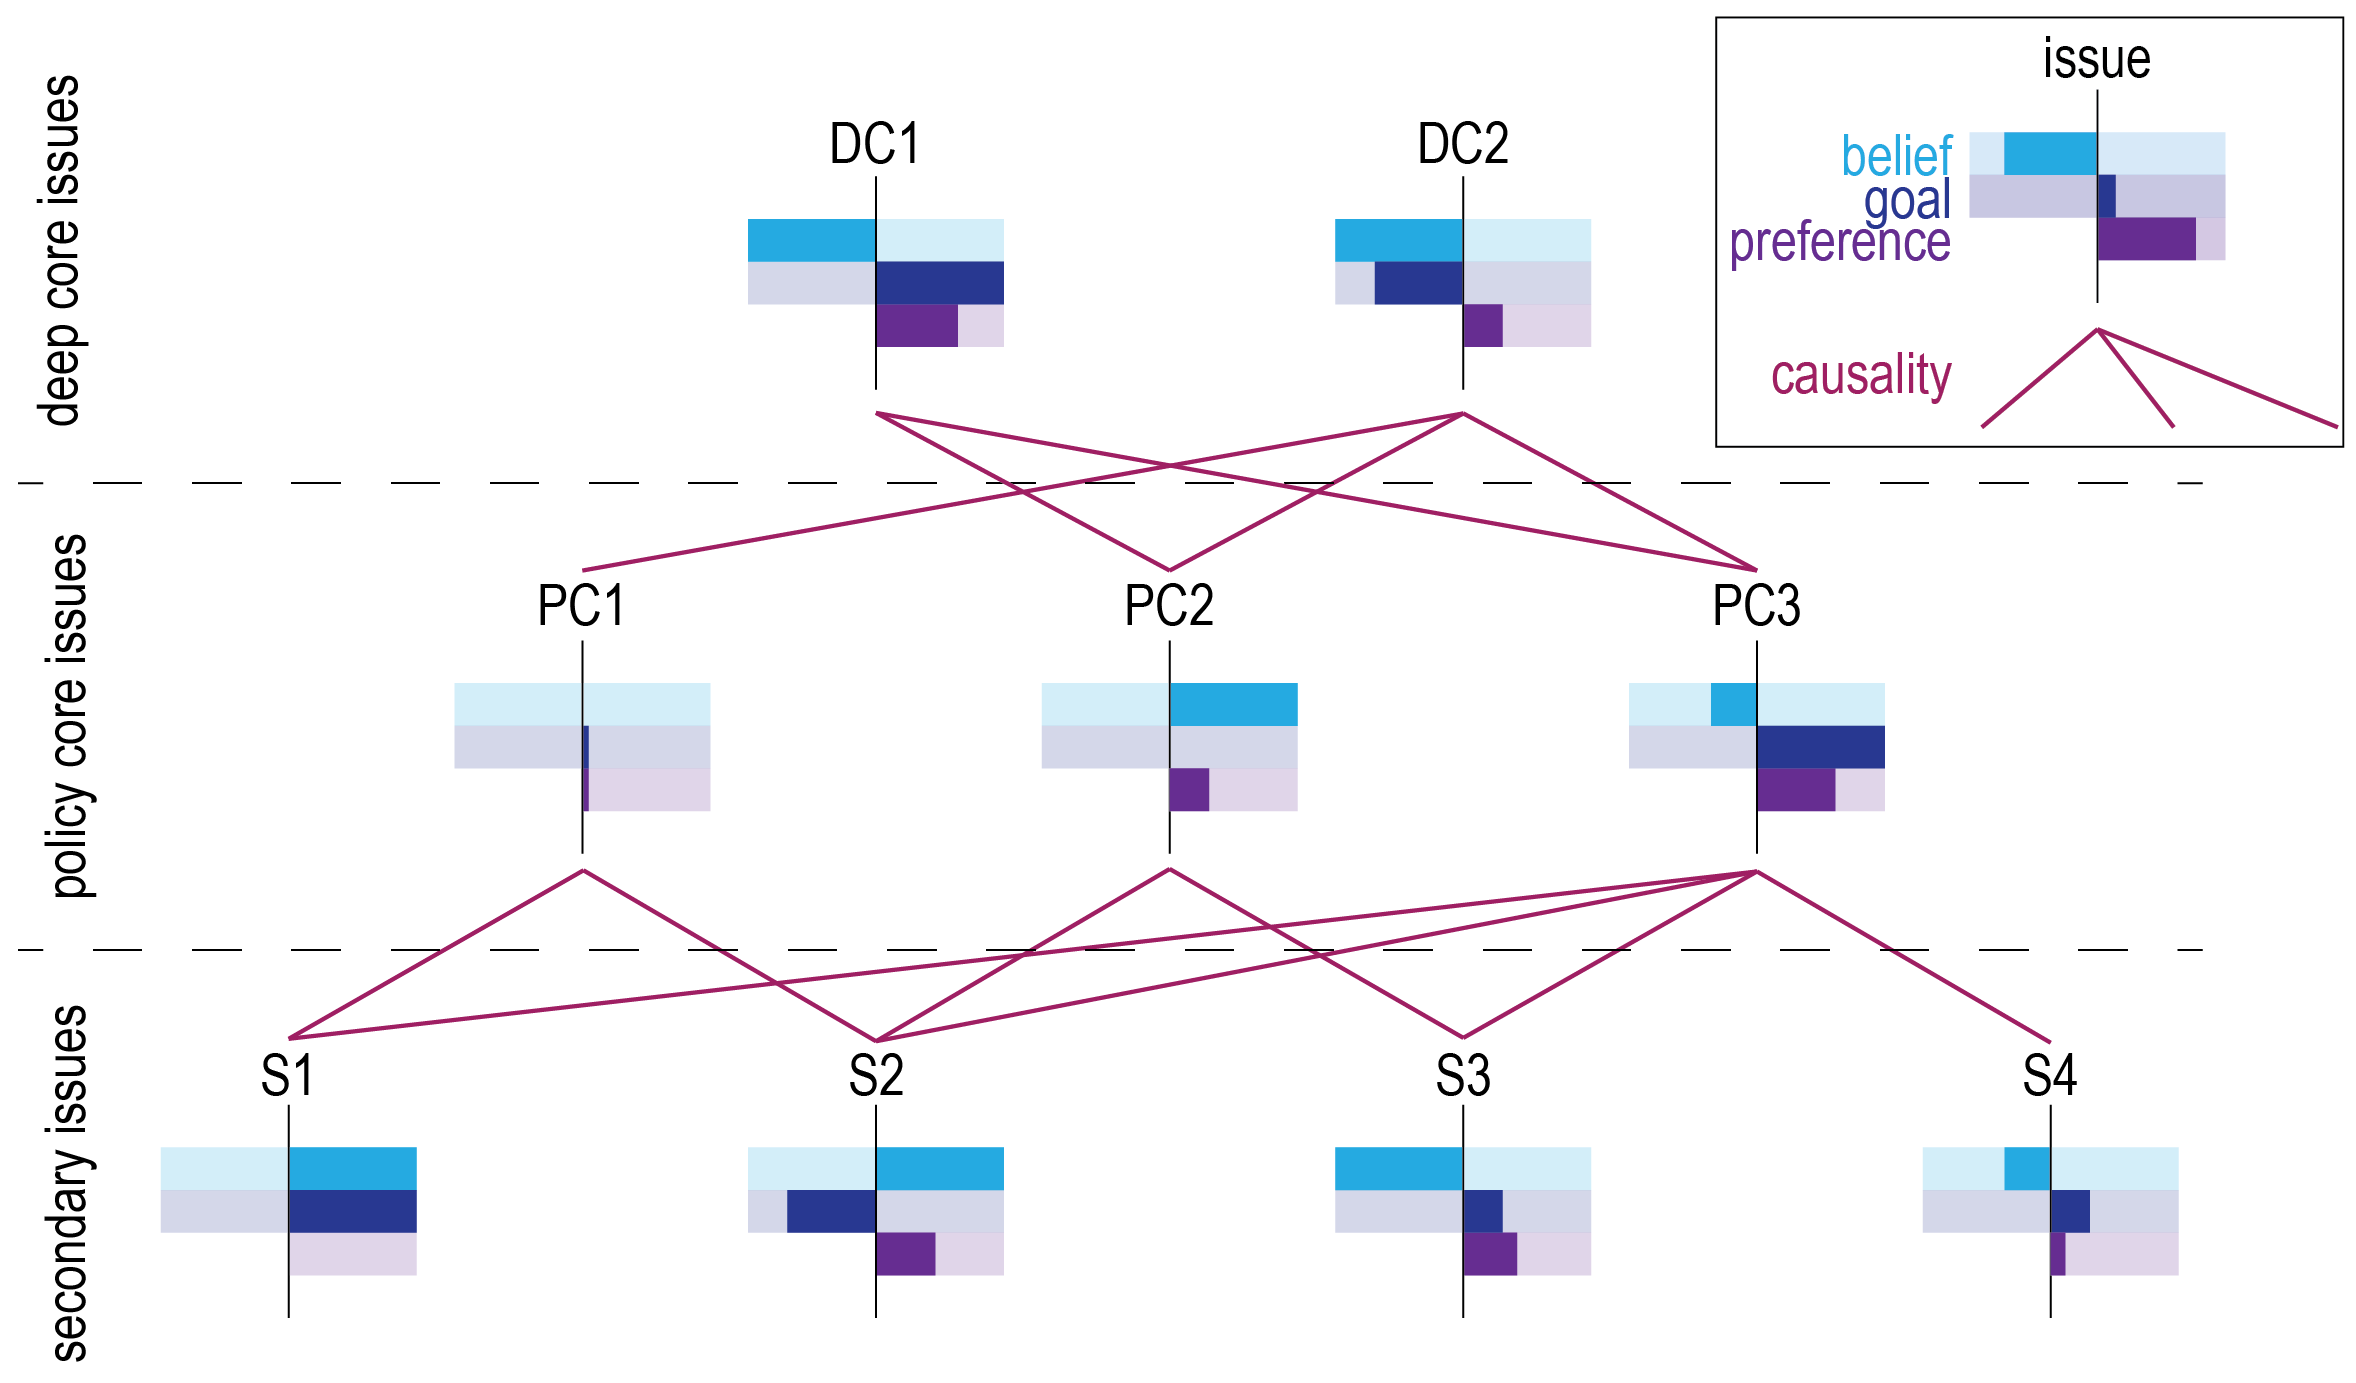
\includegraphics[width = \linewidth, angle = 0]{figures/IssueTree-01}
\caption{The issue tree structure. The issues along with their corresponding values are all arbitrary.}
\label{fig:IssueTree-01}
\end{figure}

\begin{itemize}
\item Each \emph{issue} is represented as an 6-tuple given by \texttt{issue = (ID, name, belief, goal, preference, awareness)} where
\texttt{ID} is the unique ID of the issue depending on its place in the tree,
\texttt{name} is the name of the issue,  
\texttt{belief} is the belief value of the issue, 
\texttt{goal} is the goal value of the issue, 
\texttt{preference} is the calculated preference for the issue, and
\texttt{awareness} is the boolean defining whether the issue is known to the agent or not.

\item The \texttt{belief} defines the view of the agent of a certain issue as it stands in the world. This view is subjective and can be influenced by other agents.

\item The \texttt{goal} identifies what the agent would like to see happening in the world. All actions of the agent within the policy process will be to attempt to meet his/her goals for the all the issues in his/her belief tree. This goal can be influenced by other agents within the subsystem.

\item The \texttt{preference} is a calculated parameter and it defines the urgency that the agent places on the each issues. It is calculated depending on the agent's belief, his/her goal and the causal relations linked to the issue considered. This is detailed in Section \ref{sec:prefCalcIssues}. The sum of all preference weights on any single layer of the issue hierarchy have to be equal to 1. This is so that the issues can be compared and one can be selected by the agent for advocacy purposes.

\item The \texttt{awareness} represents the fact that agents are aware of a specific issue or not. It is a boolean. If an agent is not aware of an issue, it will not consider it in any calculation, as if it did not exist. This parameter is needed for the diffusion theory where agents can become aware of certain issues based on issues considered by other agents in other subsystems \citep{berry1999innovation}.

\end{itemize}

The issue tree structure also contains causal relations. These link the issues on the different layers of the tree. They are the representation, in the agents' mind, of how each of the issues relate to one another within the system. The beliefs, goals and causal relation parameters are specified on the interval of [-1, 1] and are relative amongst all agents.

Agents have a limited attention span. This means agents have to focus on one issue at a time. This issue is selected based on perceived urgency amongst all issues. This urgency is defined as the preference of an agent and is calculated for each layer of the issue tree. Two cases must be distinguished for calculating this urgency: whether the layer considered is at the top or in the rest of the tree. The preference is calculated for each issue and the sum of all preferences on each layer must be equal to 1. The details of these calculations are provided below for the deep core, policy core and secondary issues.


%0 PREFERENCE CALCULATION (ISSUES) - Preference calculation for the deep core issues
\paragraph{Preference calculation for the deep core issues}
\label{sssec:prefDCissues}

For the top layer which is composed of the deep core beliefs, the preference is calculated differently than for the other layers. This is because these issues cannot be connected to higher layers through causal relations. The calculation of the preference for each issue is given by:

\begin{equation}
P_i = \frac{ |Go_i - Be_i|}{\sum_{j=1}^n |Go_j - Be_j|}
\end{equation}

where $j$ is defined at the number of deep core issues and $i$ characterises the deep core issue being selected for the calculation.


%0 PREFERENCE CALCULATION (ISSUES) - Preference calculation for the policy core and secondary beliefs
\paragraph{Preference calculation for the policy core and secondary beliefs}
\label{sssec:prefPCSissues}

The preference calculation for the other layers in the issue tree is adapted to include the causal relations that link these layers to higher up layers. This calculation applies to the policy core beliefs which are in the middle of the tree and the secondary beliefs at the bottom.

To calculate the preference, the gap between belief and goal for the issues is considered along with the impact of the causal relation on the gap of the issue on the above layers. The causal relations are not always helping bridge the gap between the belief and the goal of issues on a higher layer. If this is the case, then the causal relations are not considered within the calculation as there effort is counter productive within the mind of the agent. The resulting equation that can be used to calculate the preference for these layers is given by:

\begin{equation}\label{eq:preference2}
P_k= \frac{ |Go_k - Be_k| + \sum_{j=1}^n |CW_j \left( Go_j - Be_j \right)|}{\sum_{l=1}^p \left[ |Go_l - Be_l| + \sum_{j=1}^n \left|CW_{j,l} \left( Go_{j,l} - Be_{j,l} \right) \right| \right]}
\end{equation}

The sums only include these terms if $CW_j$ and $\left( Go_j - Be_j \right)$ have the same sign. If it is not the case, these terms are not considered. And where $p$ is defined at the number of policy core issues, $k$ characterises the policy core issue being selected for the calculation, $j$ specifies the associated deep core and $CW$ represents the weight of the causal relation.

Based on these preferences obtained, the agent will select one issue to advocate for as mentioned earlier. For each layer, the agent will choose the issue with the highest preference. This is the case for each layer. The actions that the agent will then perform will be to influence other agents on the issue they have selected specifically.

%%%%%%%%%%%%%%%%%%%%%%%%%%%%%%%%%%%
%- THE BELIEF SYSTEM - The policy tree
\subsection{The policy tree}
\label{ssec:policyTree}

The policy tree is designed following the example of the issue tree. An example of a structure of a policy tree is shown in \autoref{fig:TreePolicy-01}. It is composed of two main layers, corresponding to the two main steps of the policy process: the agenda setting and the policy formulation. The top layer is composed of policy families which help categorise policy instruments which are in the second layer. In the agenda setting, the agents will agree on the selection of one policy family for the agenda while the policy formulation focuses on selection a policy instrument.

\begin{figure}
\centering
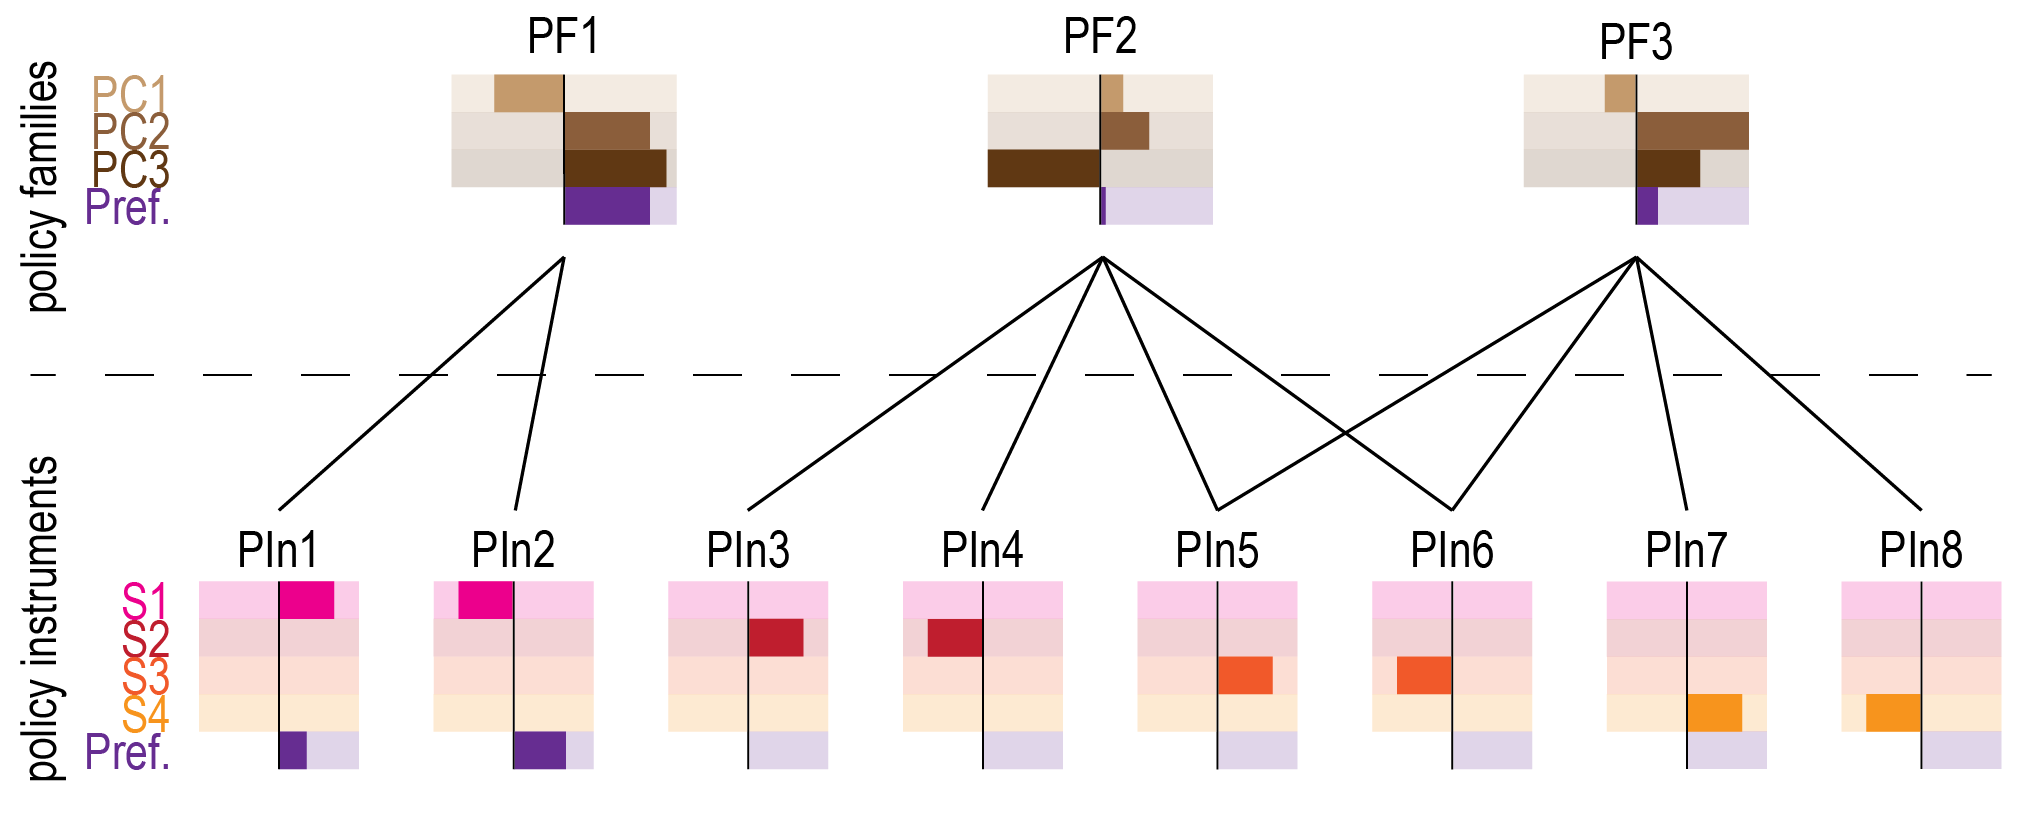
\includegraphics[width = \linewidth, angle = 0]{figures/TreePolicy-01}
\caption{The policy tree. Note that only the preferences of the policy instruments in policy family 1 are calculated as policy family one is on the agenda.}
\label{fig:TreePolicy-01}
\end{figure}

The policy families have the potential to impact the policy core issues in the issue tree. Through these potentials, the families can be graded and a preference can be established by the agents on which policy family they would like to focus on. This potential can be calculated based on a set of example policy instruments belonging to that family and their impact on the secondary issues, and through causal relations on the policy core issues in the issue tree.

The policy instruments are selected by the agents to be implemented to affect the system. They are generated by experts outside of the simulation. The policy instruments are the link between the policy process and the system. They therefore have two aspects: they have an impact on the secondary issues and they have an impact on the exogenous parameters in the system. The impact on issues is subjective and can be influenced by actors. The actual impact on exogenous parameters is set and cannot be influenced within the policy process. The policy instruments can be varied and can, through clever instrument design, also include aspects of implementation that are otherwise not present in the simulation.

Similarly to the issues in the issue tree, and due to their limited attention span, the agents have to select a policy family and a policy package at each stage of the policy process. Their choice is dependent on their perceived understanding of the impact of the policies on the issues. The more the policies have an impact on the issues and the more likely they are to be selected by the agents. The preference for each policy is also calculated in such a way that all policy preferences are equal to 1.


%- PREFERENCE CALCULATION (POLICIES) - Preference calculation for the policy families
\paragraph{Preference calculation for the policy families}
\label{sssec:prefCalcPolicyFamilies}

The preference calculation of the policy family can be decomposed in multiple parts: first there is the calculation of the potential impact of the family on each of the policy core issues according to the agent's beliefs, then there is the update of the potential impact of the policy family, and finally there is the calculation of the preference for each policy family itself.

The need to have an update step links to the possibility of being influenced on the potential impact of the policy families. To avoid losing the information and the influence from previous round, the potential impact values are not simply replaced, they are instead updated with an average between the calculation of the potential impact and the potential impact belief of the previous round.

The potential impact of a policy family is calculated using a set of dummy policy instruments. For the purpose of calculation, each policy family is populated with policy instruments that will increase by 50\% the exogenous parameter they are linked to. This leads to a 50\% increase to the secondary issues in the issue tree. This increase is then propagated to the policy core issues. These are virtually updated to see what the impact of the introduction of all policy instruments in that policy family will have on each of the policy core issue. This is compared to the current value of policy core issues. The difference is then placed, for each policy core issue, in the values of the policy families.

The potential impact of the policy family for each policy core issue is updated each time step as the average of the potential impact from the previous time step and the calculation of the new potential impact. This is done prior to performing the calculation of the preference for the policy families.

The preference for the policy family is then calculated as follows:

\begin{equation}
P_i = \frac{ \sum_{j=1}^{n} \left| \left(Go_{PC,j,i} - Be_{PC,j,i} \right) \cdot PI_{pol-fam,j,i} \right| }{ \sum_{i=1}^{m}  \sum_{j=1}^{n} \left| \left(Go_{PC,j,i} - Be_{PC,j,i} \right) \cdot PI_{pol-fam,j,i} \right|}
\end{equation}

where $PI$ is the potential impact of the policy family on a certain policy core issue, $i$ is the policy family number, $j$ is the policy core issue number, $n$ is the number of policy core issues and $m$ is the number of  policy families.

%- PREFERENCE CALCULATION (POLICIES) - Preference calculation for the policy instruments
\paragraph{Preference calculation for the policy instruments}
\label{sssec:prefCalcPolicyIns}

The preference calculation is limited to the policy instruments that fall directly within the policy family that is on the agenda. The policy instrument, having been generated by experts exogenously, are then graded by the agents based on their impact on the secondary issues. 

The equation that is used to calculate the preference is given below:

\begin{equation}
P_i = \frac{ \sum_{j=1}^{n} \left| \left(Go_{S,j,i} - Be_{S,j,i} \right) \cdot I_{pol-fam,j,i} \right| }{ \sum_{i=1}^{m}  \sum_{j=1}^{n} \left| \left(Go_{S,j,i} - Be_{S,j,i} \right) \cdot I_{pol-fam,j,i} \right|}
\end{equation}

where $i$ is the policy instrument number, $j$ is the secondary issue number, $n$ is the number of secondary issues and $m$ is the number of policy instruments. Only policy instruments that help bridge the gap between goal and belief in the issues are considered, the rest are removed.


%%%%%%%%%%%%%%%%%%%%%%%%%%%%%%%%%%%
%- POLICY VS PROBLEM FOCUSED AGENTS
\subsection{Problem and policy focused agents}
\label{ssec:selectionPolicyProblemFocus}

Once the preferences have been calculated for both the issues (at all levels) and the policies (at all levels), agents have to choose whether they will be issue focused or policy focused both in the agenda setting and the in the policy formulation phases. This is done by looking at the preferences. This is only needed for agents that are not issue or policy driven from the start. Note that an agent can be policy driven in the agenda setting phase and issue driven in the policy formulation phase. The category of the agent will affect the types of influencing action s/he can perform throughout the policy process.

To select a category, the preferences are observed. The highest preference in both the issue tree and the policy tree (at any given level depending on the step in the policy process) is recorded. Then the second highest preference is also considered. The difference between first and second is calculated. The location where the gap is highest is then considered as being more important to the agent and is therefore assigned as a category. Therefore if the policy preferences show a larger difference, then the agent will be considered to be policy driven as there is a clear sign that s/he has a strong affinity with a certain policy which is not the case for the selection of a certain issue.


%%%%%%%%%%%%%%%%%%%%%%%%%%%%%%%%%%%%%%%%%%%%%%%%%%%%%%%%%%%%%%%%%%
\section{The policy network}
\label{sec:policyNetwork}
%%%%%%%%%%%%%%%%%%%%%%%%%%%%%%%%%%%

The policy network is the network that links all agents within a subsystem. This network is composed of links with the following attributes: 

\begin{enumerate}
\item A \emph{policy network link} is represented as a 4-tuple \texttt{link = (agent1, agent2, awareness, conflictLevel)} where \texttt{agent1} and \texttt{agent2} are the agents at the end of a link, \texttt{awareness} is the awareness value, and \texttt{conflictLevel} is the conflict level characterising the relation between two agents for specific issues.

\item The \emph{awareness} value can take three main values. The value -1 refers to the fact that both agents are not aware of each other's existence. They cannot network together without external introduction from a third party. For the value 0, the actors have no connection but know each other exist. They cannot network together until they have raised their awareness level to a non-negative value through networking actions. Any positive integer relates the value of awareness between the two agents. The awareness is given on the interval $]0,1]$. Note that awareness is relative amongst all links. The policy network links between policy makers can never be -1 as policy makers are public figures (although they can be 0). Furthermore, a link cannot be downgraded to -1, it can only start at -1. As the awareness decays over time at a specific rate, there are several actions or events that can lead to a growth or stop the decay in the awareness between two agents. This is detailed later on.

\item The \emph{conflict level} parameter is determined for each agent for each issue's belief and goal, for causal relations and for each policy impact. Note that the conflict level between two agents will be different depending on which agents is considered as the conflict level is obtained based on the perception of another agent's issues. The conflict level is therefore given as a 2-tuple for each link: \texttt{(agent 1, agent 2)}. Then for each agent, the conflict level is defined per issue for the belief and then for the goal, and all causal relations. The conflict level is then calculated using:

\begin{equation}\begin{split}
CW \text{ }conflict \text{ } level_{n,n_m} &= |CW_n - CW_{n_m}| \\
belief \text{ }conflict \text{ } level_{n,n_m} &= |Be_n - Be_{n_m}| \\
goal \text{ } conflict \text{ } level_{n,n_m} &= |Go_n - Go_{n_m}| \\
impact \text{ } conflict \text{ } level_{m,n_m} &= |Im_m - Im_{n_m}|
\end{split}\end{equation}

where $CW$ the causal weight, $Go$ is the goal, $Be$ is the belief, $Im$ is the policy impact for both policy families and policy instruments, $n$ is the agent for which the conflict level is calculated and $n_m$ is the perceived value of agent $n$ on agent $m$ for that specific issue.

The resulting value is then formatted into a coefficient to be used in the grading of actions as is shown later on. When the result obtained is between 0 and 0.25, the conflict level is considered to be low, the coefficient is then set at 0.75. When the result obtained is between 0.25 and 1.75, the conflict level is considered to be medium, the coefficient is set to 0.85. Finally for a result higher than 1.75, the conflict level is considered high and the coefficient is set to 0.95. Note that both the intervals and the resulting coefficients can be varied by the modellers during experimentations to better tailor their model to their case studies.

\end{enumerate}







%%%%%%%%%%%%%%%%%%%%%%%%%%%%%%%%%%%%%%%%%%%%%%%%%%%%%%%%%%%%%%%%%%
\section{The model cycle}
\label{sec:modelCycle}
%%%%%%%%%%%%%%%%%%%%%%%%%%%%%%%%%%%

For this formalisation, it is assumed that the different rounds are performed consecutively. The agenda setting round is always performed first and is followed by the policy formulation round. This is all completed by the simulation of the system or environment. A further assumption is to assume that there is only one round of each of these steps is performed. This leads to a 3-step model with an agenda setting step, a policy formulation step and an environment simulation step. The agenda which is obtained at the end of the agenda setting helps defines what the agents will be interacting about within the policy formulation. Failure to create an agenda will lead to the bypassing of the policy formulation entirely with no implementation of any policy instruments.

The steps used to model this approach are then detailed as follows:

\begin{enumerate}
\item System simulation step:
	\begin{enumerate}
	\item \emph{System external events:} Any event that the modeller decides to implement following a scenario for the system are activated.
	\item \emph{System simulation:} The system which is exogenous to the policy process model is run to provide inputs for the next step.
	\end{enumerate}
	
\item Module interface and policy process initialisation step:
	\begin{enumerate}
	\item \emph{Update of the truth agent:} The system indicators are used to update the issue beliefs in the truth agent belief tree.
	\item \emph{Update of the beliefs:} The truth agents updates the beliefs for all agents.
	\item \emph{Policy process external events:} Any event that the modeller decides to implement following a scenario for the policy process are activated.
	\end{enumerate}
	
\item Agenda setting step:
	\begin{enumerate}
	\item \emph{Resources distribution:} Each active agent receives its resources based on his/her political affiliation.
	\item \emph{Individual agent influence actions:} All active agents perform their respective actions. The order in which the agents perform their actions is random.
	\item \emph{Agenda selection}: The agenda is made. If no agenda can be agreed on, then the policy formulation step is skipped for this cycle.
	\end{enumerate}
	
\item Policy formulation step:
	\begin{enumerate}
	\item \emph{Resources distribution:} Each active agent receives its resources based on his/her political affiliation.
	\item \emph{Individual agent influence actions:} All active agents perform their respective actions. The order in which the agents perform their actions is random.
	\item \emph{Policy package implementation:} A vote is performed. If a policy package manages to get the majority of policy makers, it is implemented in the system. If not, then nothing changes in the system and the simulation continues.
	\end{enumerate}
	
\item \emph{The simulation advances:} The simulation clock is advanced to the next tick. End of ticks actions are performed (data collection, ...).

\end{enumerate}

%- AGENDA SELECTION
\subsection{Agenda selection}
\label{ssec:agendaSelection}

The \emph{agenda} is a 2-tuple given by \texttt{agenda = (policy core issue, policy family)} where \texttt{policy core issue} is the policy core issue, seen as the problem, that is placed on the agenda and \texttt{policy family} is the policy family selected for the agenda.

The agenda can be created using one of two group of actors. Either, the policy makers are the only choosing the agenda, or it is all agents within the policy process that have a say on the agenda. The agenda is created if a majority of agents (either policy makers or all agents as mentioned before) agree on a policy core issue and a majority of agents agree on a policy family. If there is no majority, no agenda can be created. This means that that the agents cannot agree on what to discuss in general and there is no point to move into the policy formulation step. Instead, policy process proceeds directly to the environment simulation. If an agenda is agreed on, this will help narrow down the discussion within the policy formulation process by limiting the issues that can be discussed and the policy instruments that can be considered.


%- POLICY PACKAGE SELECTION AND IMPLEMENTATION
\subsection{Policy package selection and implementation}
\label{ssec:policyPackageImplementation}

In the policy formulation round, the policy makers are the agents that can select to implement a chose policy instrument. The policy instrument selection is done through a majority.

If a majority is required, 50\% plus one policy maker must select the same policy instrument. The resources of the different policy makers have no impact on this majority requirement. If a majority cannot be found, no policy instrument will not be implemented.

Within the policy formulation, there is also the possibility that a number of policy makers will not select any policy instruments as they consider none adequate enough. This would further push towards the non-implementation of any instrument.


%- EXTERNAL EVENTS
\subsection{External events}
\label{sec:externalEvents}

The external events that are considered are external events that affect the agents. External events that would affect the world such as a flood for a hydrological model are of no interest and considered out of scope of this report. However, the impact on the model such as a change in the electorate composition due to the flooding is of interest.

The following is a non-exhaustive list of potential external events which could be introduced in the model.

\begin{enumerate}
\item An election - this would create a change in the electorate representation parameter which would in turn lead to different resources allocation for the policy makers.
\item The introduction of a new issue - a new issue could be introduced to the system or to a subsystem. This would affect the knowledge parameter for an issue for all agents present in the model.
\item Resources shift - a shift in the resources distribution due to an external event could be modelled. The way the resources are attributed could be modified to simulate a crisis situation were resources are scarce. This could also be modelled as a reduction in the possibility of actions (increasing the amount of resources that is spent per action).
parameter would be changed.
\item Policy network shifts - change in the awareness parameter of specific network links.
\item Affiliation network shift - change in the affiliation coefficient parameter that defines the interaction possibilities between two different political affiliations
\end{enumerate}





%%%%%%%%%%%%%%%%%%%%%%%%%%%%%%%%%%%%%%%%%%%%%%%%%%%%%%%%%%%%%%%%%%
\section{Policy learning}
\label{sec:policyLearning}
%%%%%%%%%%%%%%%%%%%%%%%%%%%%%%%%%%%
Policy learning is a concept from the ACF where the belief system of agents evolve over time due to interaction with one another and with the environment. Such concept is emulated in this model through actions that agents can perform on one another. These are split in two main categories: the general actions which are mandatory and cannot be selected and the targeted actions. These targeted actions are selected by the agents as being the best actions they can perform to reach their goals. Overall, it is these interactions between the agents that lead to the emergent phenomenon of policy learning.

%- GENERAL ACTIONS
\subsection{General actions}
\label{ssec:}

The general actions are actions that are mandatory to perform. They tend to be performed each cycle and tend to relate the passive agents to the active ones. This therefore includes the influencing of the external parties on the electorate, the transmissions of the real world data to all actors - affecting their beliefs -, and the influencing of the electorate on the policy makers' issues. These actions are necessary to update the agents on what is going on in the real world. They are also needed to loop in the electorate and outline their impact on the overall system and the direction of the policy process.

%0 THE ACTIONS - TRUTH AGENT - Transmitting the states
\paragraph{Update of the agents' issue beliefs}
\label{sssec:actionEPs}

The truth agent updates the beliefs of all of the agents within the policy process. The equation for this is given as follows.

\textcolor{red}{Come up with a reasonable equation that is not an average.}

\begin{equation}
Be_{agent} := Be_{agent} + \frac{1}{n} \sum_{i=1}^n \left( \left(Be_{EP_n} - Be_{agent} \right) \cdot affiCoef_{Aff_n,Aff_m} \right)
\end{equation}


%- TARGETTED AGENT ON AGENT ACTIONS
\subsection{Targeted actions}
\label{ssec:}

Targeted actions are the main driver of policy learning within the policy process. These targeted actions are initiatives from the agents to influence, lobby or convince other agents within their network. Such influence is aim at changing the beliefs of others such that each agent is able to push issues or policies that are important to him/her onto the agenda and ultimately, have certain preferred policy instrument implemented.

The influencing actions affects all parts of the belief system of the actors both in the issue and the policy trees. Five main actions are considered in this respect. Within the issue tree, the agents can influence the goals, the beliefs and the causal relations of other agent's belief system. Within the policy tree, the agents can influence the perceived impact of the policy families and the policy instruments of other agents.

Because of the number of actions at their disposition, the agents have to select which action they want to perform. They are not able to perform all actions possible due to limited resources. For this, and within this formalisation, the agents will grade all their possible actions. The grade is entirely based on their conflict level with other agents, their affiliation differences (or lack thereof) and their awareness of other agents. Based on this grade, they will decide to implement the action that they think will bear the most weight on the other agent. The action impact will then be based on the difference in beliefs between the two agents, the resources spent and the affiliation of the two agents.

Not all agents perform the same targeted actions. The external parties are considered to be different from the policy entrepreneurs and the policy makers. External parties are conceptualised as agents that have a larger reach. The actions they perform therefore affect all agents within their network at once and not only one agent at a time. This affects slightly the grading of their actions but the equations used remain the same overall. Only the impact of their actions is divided by the number of agents they are influencing at the same time.


%0 ISSUE VS PROBLEM FOCUSED
\paragraph{Issue versus policy focused actions}
\label{sssec:}

The actions of the actors have to be targeted - as the title suggests. This targeting will depend on whether an actor is issue or policy driven. If an actor is issue driven, all his/her actions will focus on making other actors understand that the issue s/he has selected is an important one to tackle. With this in mind, the agent will attempt to influence other actors such that the gap within their belief system for that issue, that is the difference between the belief and the goal of that issue, will widen. Actions will also target policies that can affect this gap, and the agent will attempt to convince other agents on policies that are most effective at solving that issue.

Similarly, for agents that are policy driven, they will attempt to convince other actors that the policy they have selected is a solution to all their problems. For this, they will perform actions that promote their policies by boosting their perceived impact on issues that are considered prominent by other actors. They will also perform influencing actions on issues where the policies they have chosen are more likely to have an impact by widening the gap between belief and goal for these issues.

Overall, this means that although the equations are similar for both categories of agents for the actions, the way these equations are used and targeted at other agents will depend on whether an agent is issue or policy focused. The actions are the same, their aims are different.


%0 EQUATIONS LIKELIHOOD
\paragraph{The likelihood equations for issue focused agents}
\label{sssec:}

When performing an action, an agent will first grade all the possible action s/he can perform. The grading is different for each action and the equations are provided for all actions below.

For goal direct influence:

\begin{equation}\label{eq:likelihoodAimChange}
G_{Go, n_m} = conflictLevel_{Go, n, m} \cdot awareness_{n,m} \cdot actionWeight_{n,m}
\end{equation}

where $G$ stands for the grade, $n$ is the influencing agent, $m$ is the influenced agent. $n_m$ is the perfection of the beliefs of the influenced agent by the influencing agent and $CW$ is the causal weight of the causal relation.

For belief direct influence:

\begin{equation}\label{eq:likelihoodStateChange}
G_{Be, n_m} = conflictLevel_{Be, n,m} \cdot awareness_{n,m} \cdot actionWeight_{n,m}
\end{equation}

where $G$ stands for the grade, $n$ is the influencing agent, $m$ is the influenced agent. $n_m$ is the perfection of the beliefs of the influenced agent by the influencing agent and $CW$ is the causal weight of the causal relation.

For framing:

\begin{equation}\label{eq:likelihoodFraming}
G_{CW, n_m} = conflictLevel_{CW, n, m} \cdot awareness_{n,m} \cdot actionWeight_{n,m}
\end{equation}

where $G$ stands for the grade, $n$ is the influencing agent, $m$ is the influenced agent. $n_m$ is the perfection of the beliefs of the influenced agent by the influencing agent and $CW$ is the causal weight of the causal relation.

For the framing actions, the grading is done on all causal relations that link to the issue selected by the agent. This can result in several grades being obtained and considered by the agent.

%0 EQUATIONS LIKELIHOOD
\paragraph{The likelihood equations for policy focused agents}
\label{sssec:}

For policy family influence (only in the agenda setting step):

\begin{equation}\label{eq:likelihoodPFchangePolicy}
G_{PF_{l}, n_m} = \frac{1}{p} \sum_{j=1}^{p} conflictLevel_{PI_{l,j}, n,m} \cdot awareness_{n,m} \cdot actionWeight_{n,m} 
\end{equation}

For policy instrument influence (only for the policy formulation step):

\begin{equation}\label{eq:likelihoodPFchangeProblem}
G_{PIns, n_m} = \frac{1}{p} \sum_{l=1}^{q} conflictLevel_{PI_{l,j}, n,m} \cdot awareness_{n,m} \cdot actionWeight_{n,m} 
\end{equation}

where $n$ is the agent influencing, $m$ is the agent being influenced, $j$ is the secondary issue number, $p$ is the number of secondary issues and $l$ is the policy instrument number (selected by the agent).

%0 EQUATIONS IMPACT
\paragraph{The impact equations for issue focused agents}
\label{sssec:}

The actions impact will then vary depending on the action that is being considered. The equations used to calculate these impacts are presented below.

For goal direct influence:

\begin{equation}\label{eq:impactAimChange}
Go_{m} := Go_{m} + \left(Go_{n} - Go_{m} \right) \cdot resources
\end{equation}

For belief direct influence:

\begin{equation}\label{eq:impactStateChange}
Be_{m} := Be_{m} + \left(Be_{n} - Be_{m} \right) \cdot resources
\end{equation}

For framing:

\begin{equation}\label{eq:impactFraming}
CW_{m} := CW_{m} + \left(CW_{n} - CW_{m} \right) \cdot resources
\end{equation}

For (issue focused agents) policy family influence (only in the agenda setting step):

\begin{equation}\label{eq:impactPFChangeProblem}
PI_{l,j,m} := PI_{l,j,m} + \left(PI_{l,j,n} - PI_{l,j,m} \right) \cdot resources
\end{equation}

where $j$ is the policy core issue number, $l$ is the policy family number (selected by the agent), $m$ is the agent being influenced. Note that for the problem focused agents, the policy family is changed but the policy core issue number remains constant.

%0 EQUATIONS IMPACT
\paragraph{The impact equations for policy focused agents}
\label{sssec:}

For policy family influence (only in the agenda setting step):

\begin{equation}\label{eq:impactPFChangePolicy}
PI_{l,j,m} := PI_{l,j,m} + \left(PI_{l,j,n} - PI_{l,j,m} \right) \cdot resources \cdot affiCoef_{Aff_n,Aff_m}
\end{equation}

where $j$ is the policy core issue number, $l$ is the policy family number (selected by the agent), $m$ is the agent being influenced. Note that for the policy focused agents, the policy family remains constant but the policy core issue number is changed.

For policy instrument influence (only in the agenda setting step):

\begin{equation}\label{eq:impactPFChangeProblem}
PI_{l,j,m} := PI_{l,j,m} + \left(PI_{l,j,n} - PI_{l,j,m} \right) \cdot resources \cdot affiCoef_{Aff_n,Aff_m}
\end{equation}

where $j$ is the secondary issue number, $l$ is the policy instrument number (selected by the agent), $m$ is the agent being influenced.


%%%%%%%%%%%%%%%%%%%%%%%%%%%%%%%%%%%%%%%%%%%%%%%%%%%%%%%%%%%%%%%%%%
\appendix
%%%%%%%%%%%%%%%%%%%%%%%%%%%%%%%%%%%%%%%%%%%%%


%%%%%%%%%%%%%%%%%%%%%%%%%%%%%%%%%%%%%%%%%%%%%%%%%%%%%%%%%%%%%%%%%%
\bibliographystyle{apalike} 
\bibliography{references}
%%%%%%%%%%%%%%%%%%%%%%%%%%%%%%%%%%%%%%%%%%%%%

\end{document}
